\documentclass[a4paper]{article}
\usepackage {changepage}
\usepackage{fancyhdr}

\usepackage {fontspec}
\pagestyle{fancy}
\setromanfont{Lantinghei SC Extralight}
\setmonofont{Courier New}
\XeTeXlinebreaklocale ``zh''
\XeTeXlinebreakskip = 0pt plus 1pt
\textheight = 650pt
\begin{document}
\title{实验报告 Lab 2}
\author{姓名:王钦\quad 学号:13349112}
\date{}
\maketitle

\section*{ A first look at the captured trace}
\hangindent=4em \hangafter=-200{
	1. Client IP:\verb| 192.168.1.102|,Client Port:\verb| 1161| \\\\
	{\centering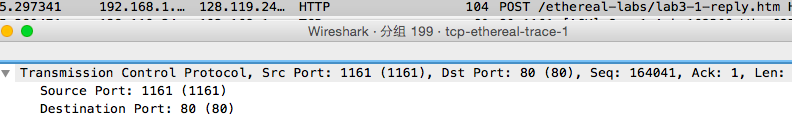
\includegraphics[scale=0.5]{Illustrations/1_1.png}}\\\\
	{\centering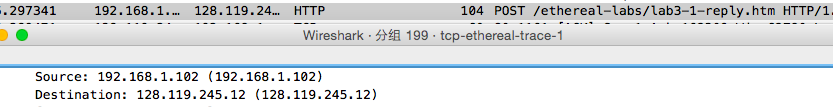
\includegraphics[scale=0.5]{Illustrations/1_2.png}}\\\\
	2. IP address of gaia.cs.umass.edu:\verb| 128.119.245.12| ,Port: \verb| 80|\\\\
	{\centering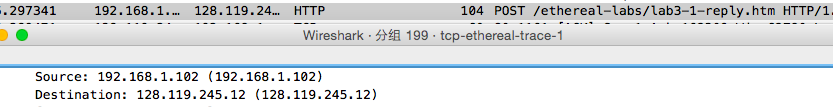
\includegraphics[scale=0.5]{Illustrations/1_2.png}}\\\\
	{\centering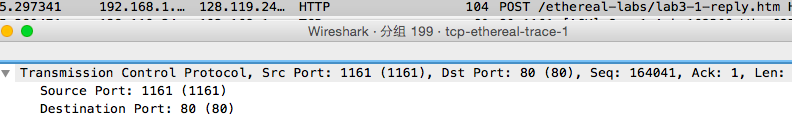
\includegraphics[scale=0.5]{Illustrations/1_1.png}}\\\\
	3. I use \verb|wget| to download alice.txt and upload.And my computer client IP: \verb| 192.168.41.115|,Souce Port: \verb|52685|\\\\
	{\centering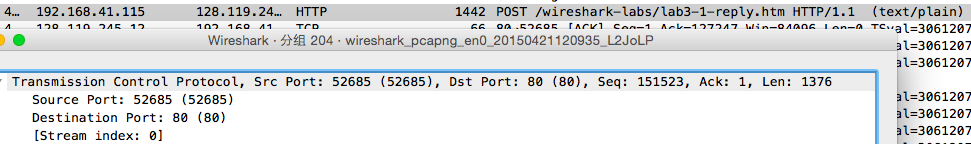
\includegraphics[scale=0.5]{Illustrations/3.png}}\\\\
}
\section*{ Tcp Basics}
\hangindent=4em \hangafter=-200{
	4. Sequence Number is : \verb|0|,In flags of identifies note the Syn is set,ackledgment is 
	not-set ( note:I am not use the tcp-ethereal-trace-1 in wireshark- traces.zip)\\\\
	{\centering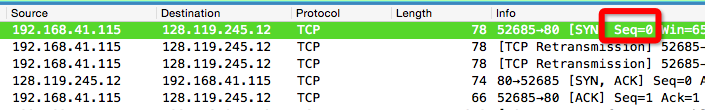
\includegraphics[scale=0.5]{Illustrations/4_1.png}}\\\\
	{\centering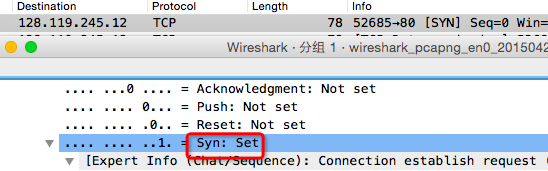
\includegraphics[scale=0.5]{Illustrations/4_2.png}}\\\\
	5. Sequence Number is : \verb|0|.ACKnowledgement number is 1.Determine this value by last TCP SYN segment:\verb| ACKnowledgement value= initiate sequence number of the TCP SYN segment+1 |.In flags of identifies note the Syn is set,ackledgment is set\\\\
	{\centering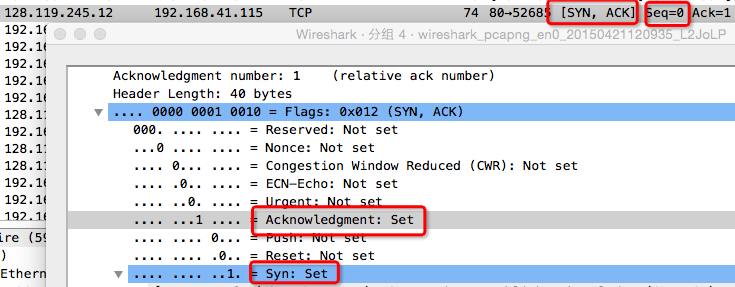
\includegraphics[scale=0.5]{Illustrations/5.png}}\\\\
	6. The sequence number of the TCP segment containing the HTTP POST command : \verb| 1|.\\\\
	{\centering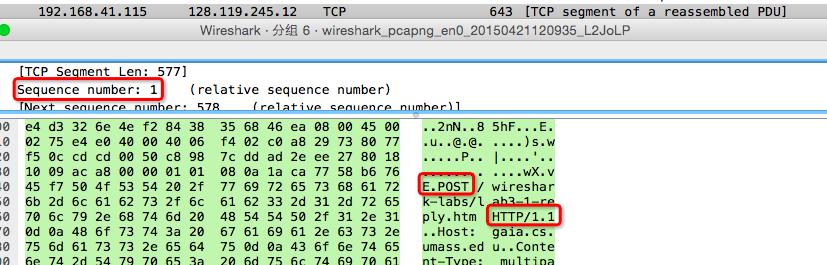
\includegraphics[scale=0.5]{Illustrations/6.png}}\\\\
	7. The first six \verb| [No,sequence number]| see below chart\\\\
	\begin{tabbing}
	  \hspace{4em} No.\hspace{4mm} \= Sequence number \\
	  \hspace{4em}	6 \> 1    \\
	  \hspace{4em}	7 \> 578  \\
	  \hspace{4em}	8 \> 715  \\
	  \hspace{4em}	9 \> 2143  \\
	  \hspace{4em}	11 \> 3571  \\
	  \hspace{4em}	14 \> 4999  \\
	\end{tabbing}
	The first six \verb| [No,time segment send,time ACK segment received,RTT]| see below chart\\\\
	\begin{tabbing}
	 \hspace{4em}	No.	\hspace{4mm} \= Time send. \hspace{4mm} \= Time ACK received  \hspace{4mm} \= RTT(seconds) \\
	 \hspace{4em}	6 \>2.355753000	\> 2.661392000 \> 0.3056390 \\
	 \hspace{4em}	7 \>2.364271000	\> 2.661392000 \> 0.2971210 \\
	 \hspace{4em}	8 \>2.365312000	\> 2.662281000 \> 0.2969690 \\
	 \hspace{4em}	9 \>2.365313000	\> 2.662288000 \> 0.296975 \\
	 \hspace{4em}	11 \>2.661491000 \> 2.905288000 \> 0.243797 \\
	 \hspace{4em}	14 \>2.662481000 \> 2.917857000 \> 0.255376 \\
	\end{tabbing}
	Determine the formula :\\ \verb|EstimatedRTT = 0.875 * EstimatedRTT + 0.125 * SampleRTT|.\\The first six \verb| [No, EstimatedRTT]| see below chart\\\\
	\begin{tabbing}
	 \hspace{4em}	No.	\hspace{4mm} \= EstimatedRTT(seconds)\\
	 \hspace{4em}	6 \>0.3056390\\
	 \hspace{4em}	7 \>0.30457425\\
	 \hspace{4em}	8 \>0.297102\\
	 \hspace{4em}	9 \>0.29696975\\
	 \hspace{4em}	11 \>0.29032775\\
	 \hspace{4em}	14 \>0.245244375\\
	\end{tabbing}
	Snapshot:\\\\
	{\centering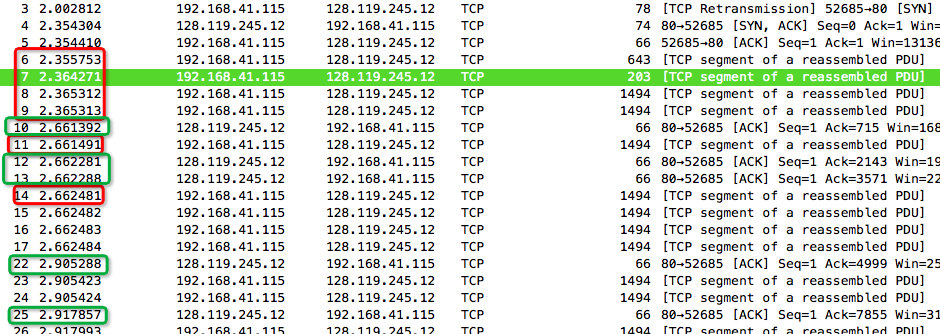
\includegraphics[scale=0.5]{Illustrations/7_1.png}}\\\\
	{\centering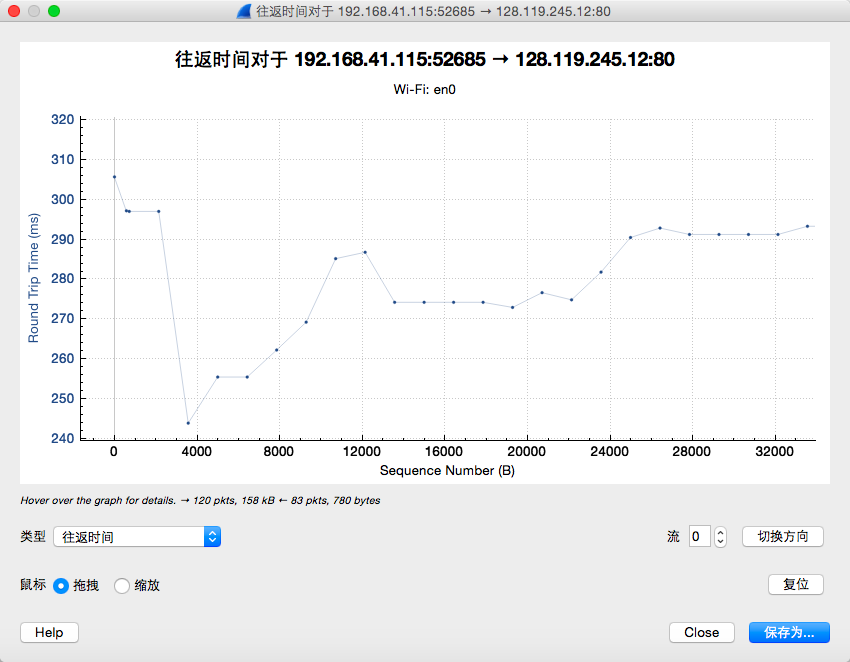
\includegraphics[scale=0.5]{Illustrations/7_2.png}}\\\\
	8. The length of first TCP package is \verb|577 bytes|,The 5 rest is \verb|1428 bytes|\\\\
	{\centering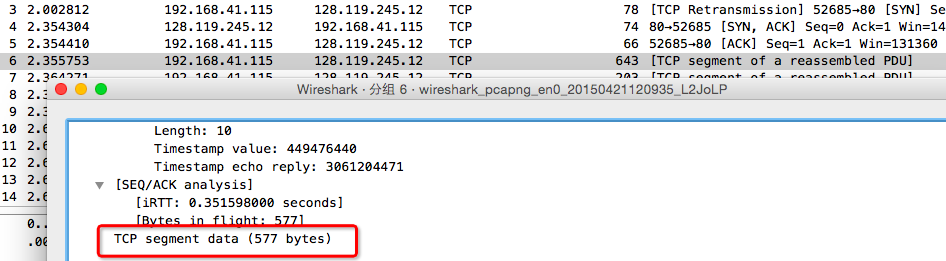
\includegraphics[scale=0.5]{Illustrations/8_1.png}}\\\\
	{\centering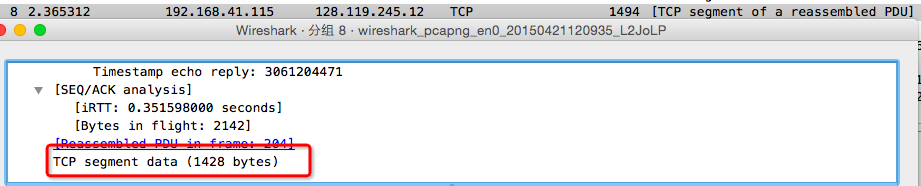
\includegraphics[scale=0.5]{Illustrations/8_2.png}}\\\\
	9. The minimum amount of available buffer space: \verb|14480|.No, sender is never throttled due to lacking of receiver buffer\\\\
	{\centering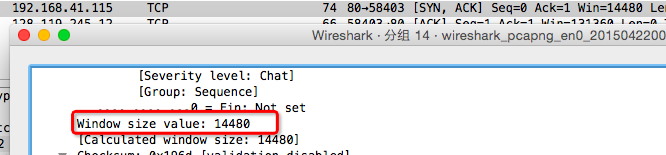
\includegraphics[scale=0.5]{Illustrations/9.png}}\\\\
	10. Yes,there has some retransmitted segment.I check it by \verb|Statistics->TCP Stream Graph- >Time/Sequene Graph.| And I find some decrease.\\\\
	{\centering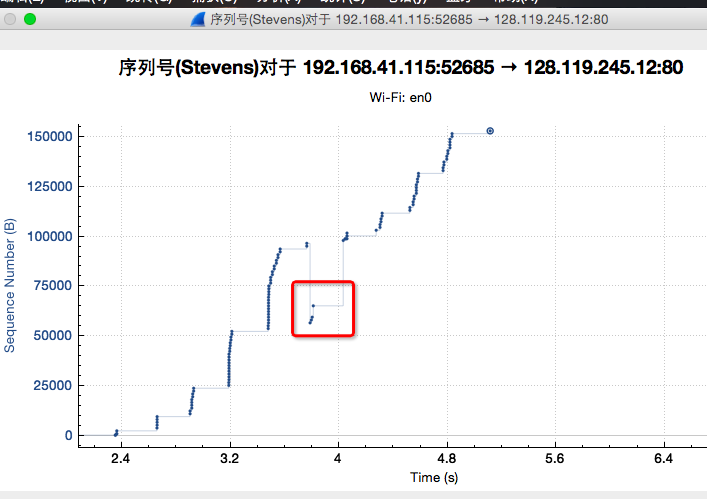
\includegraphics[scale=0.5]{Illustrations/10.png}}\\\\
	11. Amount data doesn't first is 137,subsequence are 1428,There cases in below table.\\\\ 
	\begin{tabbing}
	 \hspace{4em}	No.\hspace{4mm} \= Acknowledged sequence number\hspace{4mm} \= Acknowledged data \\
	 \hspace{4em}	8 \>578 \>137\\
	 \hspace{4em}	10 \>715 \>1428\\
	 \hspace{4em}	12 \>2143 \> 1428\\
	 \hspace{4em}	13 \>3571 \> 1428\\
	 \hspace{4em}	22 \>4999 \> 1428\\
	 \hspace{4em}	25 \>7855 \> 1428\\
	 \hspace{4em}	30 \>9283 \> 1428\\
	\end{tabbing}
	12. The first segment size when start transmit data, sequence is \verb| 1 | mean 1 byte.And the last sequence is \verb |164091| ,we conclude follow figures\\
	\verb| amount data = 164091 - 1 = 16490 bytes|\\
	\verb| amount time = 4.836206 - 2.355753 = 2.480453 sec| \\
	\[ throughput = \frac{amount \ data}{amount \ time} = \frac{ 164090}{2.480453} = 66153.23894466052 \ bytes/s\] \\\\
	13. At point A the begin of slow start ,point B is end of slow start then TCP use additive-Increase approach because the \verb|CongWin| reaches \verb|Threshold|.So point B is the begin of congestion avoidance take over.Until at point C sender had received three duplicate ACKs,TCP use multiplicative decrease,\verb|Threshold| is set to one half of the current \verb|ConWin|.So point D is the end of congestion avoidance phase,then \verb|CongWin| will ramps up linearly.\\\\ 
	{\centering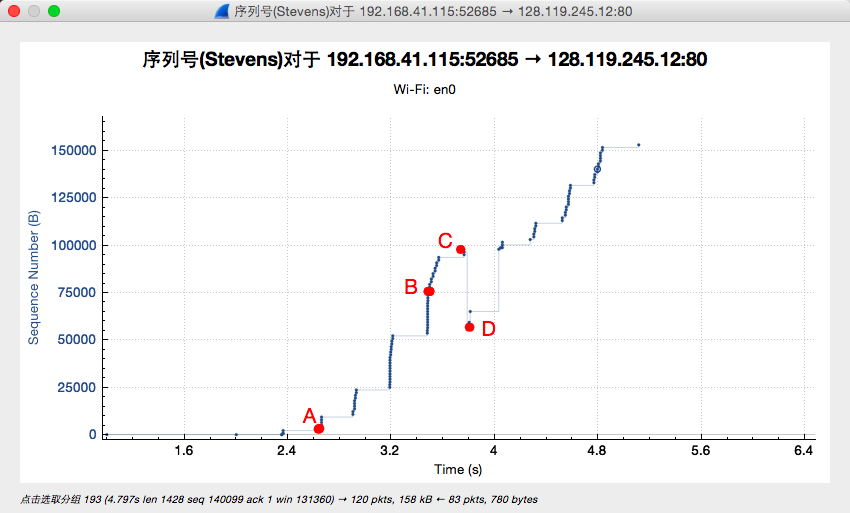
\includegraphics[scale=0.5]{Illustrations/13_2.png}}\\\\
	From below figure we can see after three duplicate ACKs,maybe the seq 56407 is lost,then client send a fast retransmission.And TCP use multiplicative decrease 
	approach.		\\\\
	{\centering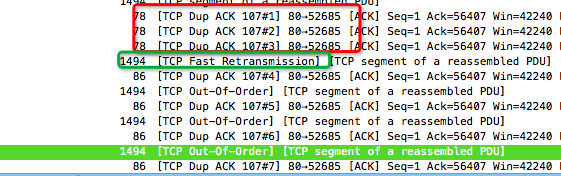
\includegraphics[scale=0.5]{Illustrations/13_1.png}}\\\\
	14. At point A the begin of slow start ,point B is end of slow start then TCP use additive-Increase approach because the \verb|CongWin| reaches \verb|Threshold|.So point B is the begin of congestion avoidance take over.Until at point C sender had received three duplicate ACKs,TCP use multiplicative decrease,\verb|Threshold| is set to one half of the current \verb|ConWin|.So point D is the end of congestion avoidance phase,then \verb|CongWin| will ramps up linearly.\\\\ 
	{\centering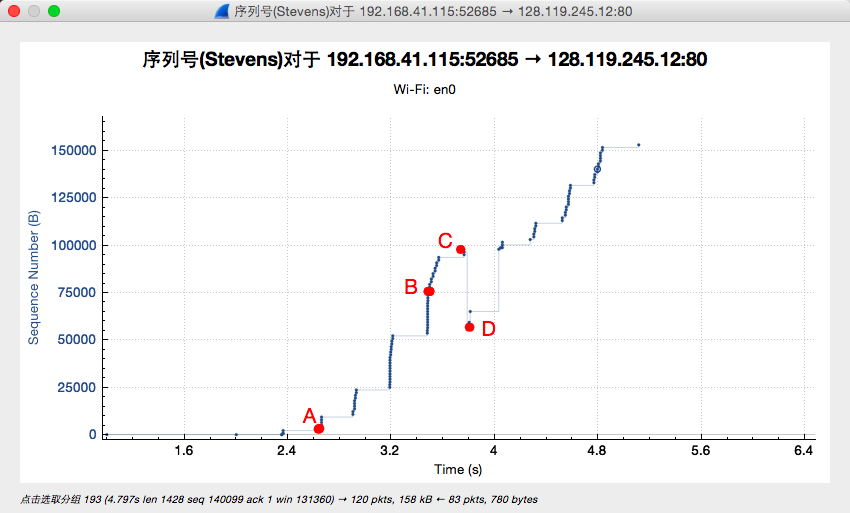
\includegraphics[scale=0.5]{Illustrations/13_2.png}}\\\\
	From below figure we can see after three duplicate ACKs,maybe the seq 56407 is lost,then client send a fast retransmission.And TCP use multiplicative decrease 
	approach.		\\\\
	{\centering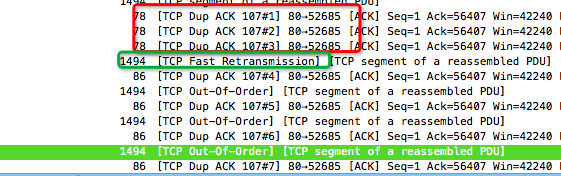
\includegraphics[scale=0.5]{Illustrations/13_1.png}}\\\\





}

\fancyfoot[OC]{ \footnotesize{https://github.com/wangqin4377/Homework\_Wangqin/tree/master/network/}}
\end{document}


